202. \begin{figure}[ht!]
\center{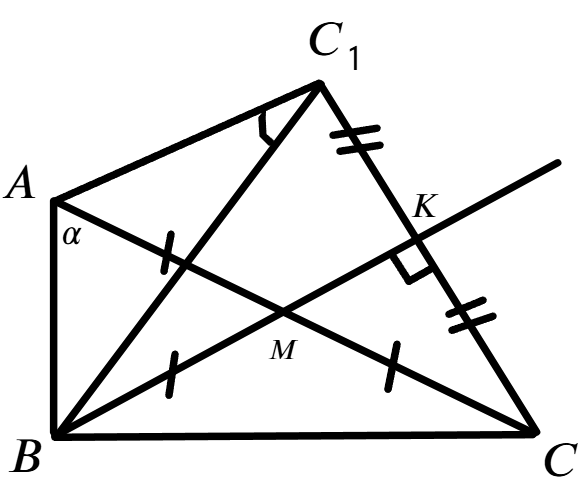
\includegraphics[scale=0.35]{g9-201.png}}
\end{figure}\\
Так как $BM$ --- медиана, а точка $C_1$ симметрична точке $C,$ точки $M$ и $K$ являются серединами отрезков $AC$ и $CC_1$ соответственно. Тогда $MK$ является средней линией в треугольнике $ACC_1,$ а значит $MK\parallel AC_1$ и $\angle AC_1B=\angle C_1BK$ как накрест лежащие. Так как в прямоугольном треугольнике медиана, проведённая из прямого угла, равна половине гипотенузы, верно равенство $BM=MC,$ а значит треугольник $BMC$ равнобедренный и $\angle MBC=\angle MCB=90^\circ-\alpha.$ Так как точки $C_1$ и $C$ симметричны, верно равенство $BC_1=BC,$ а значит треугольник $BCC_1$ равнобедренный и $BK$ является не только высотой и медианой, н и биссектрисой, поэтому $\angle C_1BK=\angle KBC=90^\circ-\alpha,$ таким образом и $\angle AC_1B=90^\circ-\alpha.$\\
